% vim: set foldmethod=marker foldlevel=0:

\documentclass[a4paper]{article}
\usepackage[UKenglish]{babel}

\usepackage{preamble}

\usepackage{graphicx}
\graphicspath{ {./imgs/} }

\title{MA144 Methods of Mathematical Modelling 2, Assignment 1}
\author{Dyson Dyson}
\date{}

\begin{document}

\maketitle

\setlength{\parindent}{0em}
\setlength{\parskip}{1em}

% {{{ Q1
\question{1}

\subsection{~}

The polar curve with equation $r = f(\theta)$ can be parametrised as $\ul r (\theta) = (f(\theta) \cos \theta, f(\theta) \sin \theta)$. Then $$\dd{\ul r}\theta = \l(\dd f\theta (\theta) \cos \theta - f(\theta) \sin \theta, \dd f\theta (\theta) \sin \theta + f(\theta) \cos \theta\r)$$
Therefore \begin{align*}
\| \ul r\,'(\theta) \| &= \sqrt{\l( f'(\theta) \cos \theta - f(\theta) \sin \theta \r)^2 + \l( f'(\theta) \sin \theta + f(\theta) \cos \theta \r)^2}\\[1ex]
&= \sqrt{f'(\theta)^2 \cos^2 \theta - 2 f(\theta) f'(\theta) \cos\theta \sin\theta + f(\theta)^2 \sin^2 \theta}\\[1ex]
&\phantom{=} \overline{+ f'(\theta)^2 \sin^2 + 2 f(\theta) f'(\theta) \cos\theta \sin\theta + f(\theta)^2 \cos^2 \theta}\\[1ex]
&= \sqrt{f'(\theta)^2 (\cos^2 \theta + \sin^2 \theta) + f(\theta)^2 (\cos^2 \theta + \sin^2 \theta)}\\[1ex]
&= \sqrt{f'(\theta)^2 + f(\theta)^2}\\[1ex]
&= \sqrt{\l(\dd f\theta\r)^2 + f^2}\\[1ex]
\end{align*}

Therefore the arc length of the curve is $$s = \intlim ab {\sqrt{\l(\dd f\theta\r)^2 + f^2}}\theta$$ as required.

\subsection{~}

Let $r = 1 + \cos\theta$. %Then $\ul r(\theta) = (\cos\theta + \cos^2\theta, \sin\theta + \sin\theta\cos\theta)$.

% TODO: Sketch the curve
% 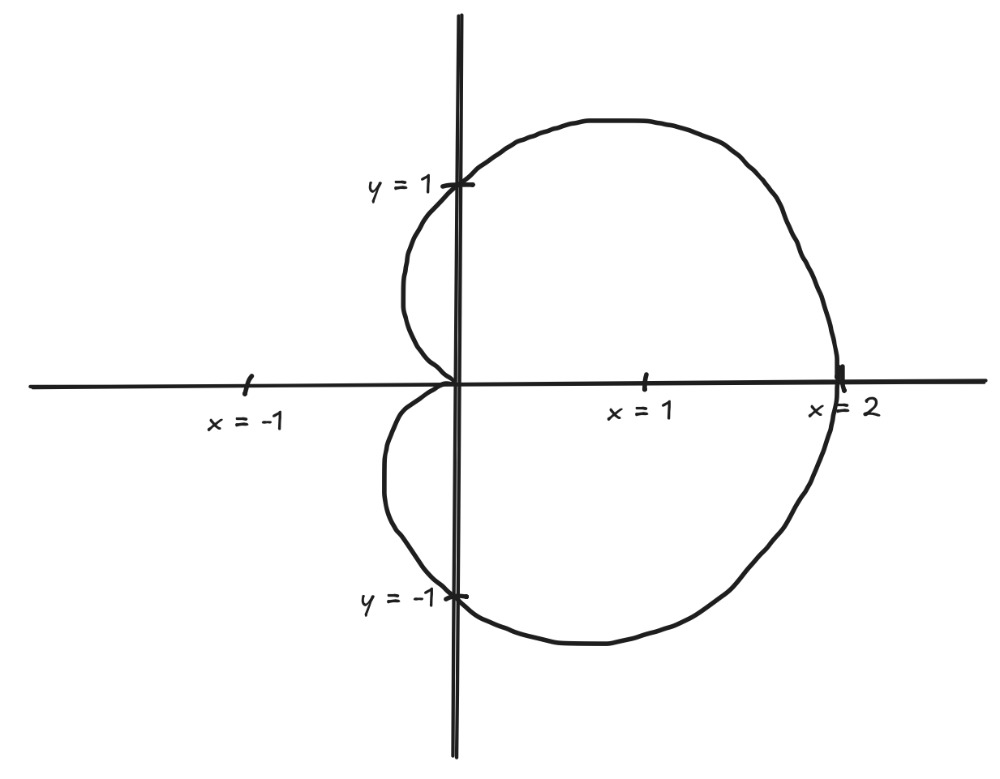
\includegraphics[scale=0.4]{Q1b}

$\ds\dd r\theta = -\sin\theta$ so the arc length is \begin{align*}
s &= \intlim 0{2\pi} {\sqrt{\sin^2 \theta + (1 + \cos\theta)^2}} \theta\\[1ex]
&= \intlim 0{2\pi} {\sqrt{\sin^2 \theta + 1 + 2\cos\theta + \cos^2 \theta}} \theta\\[1ex]
&= \intlim 0{2\pi} {\sqrt{2 + 2\cos\theta}} \theta
\end{align*}
I don't know how to do this integral but apparently it's $4\pi$.

\subsection{~}

The curve given by $r = 1 + \cos k\theta$ is non-simple whenever $k$ is not an integer.
% }}}

% {{{ Q2
\question{2}

\subsection{~}
\subsection{~}
\subsection{~}
% }}}

% {{{ Q3
\question{3}

\subsection{~}
\subsection{~}
% }}}

\end{document}
